\documentclass[review]{elsarticle}

\usepackage{lineno,hyperref}
\modulolinenumbers[5]

\journal{NDT\&E International}

\usepackage{amsmath}
\usepackage{graphicx}
\usepackage{booktabs}
\usepackage{multirow}
\usepackage{xcolor}
\usepackage{subcaption}
\usepackage{algorithm}
\usepackage{algpseudocode}
\usepackage{siunitx}

\graphicspath{{figures/}}

\begin{document}

\begin{frontmatter}

\title{STFT-Based Condition-Aware CNN with Conditional GAN Augmentation for Multi-Depth Soil Moisture Prediction from GPR A-Scans}

\author[rut]{Tianjie Zhang}
\author[rut]{[Advisor Name]}

\address[rut]{Department of Civil and Environmental Engineering, Rutgers, The State University of New Jersey, Piscataway, NJ 08854, USA}

\begin{abstract}
Accurate monitoring of soil moisture beneath pavements and around buried pipelines is critical for infrastructure integrity assessment, yet existing methods either require invasive sensor installation or provide only point measurements. Ground-penetrating radar (GPR) offers a non-invasive alternative, but extracting reliable moisture estimates from GPR A-scan signals remains challenging due to complex wave propagation effects and limited labeled datasets. This paper proposes a machine learning pipeline for simultaneous multi-depth soil moisture prediction from single-pass GPR A-scans. The pipeline comprises three components: (1) Short-Time Fourier Transform (STFT) signal representation, which converts each A-scan into a 2D time-frequency spectrogram where moisture-related dielectric and attenuation effects are spatially separated; (2) a condition-aware convolutional neural network (CA-CNN) that jointly encodes the STFT image with known deployment metadata (soil type and pipe diameter) via one-hot feature concatenation; and (3) a conditional Wasserstein GAN with gradient penalty (cWGAN-GP) that augments the training set by generating physically plausible synthetic A-scans conditioned on soil type, pipe diameter, and moisture labels. Experiments are conducted on a controlled sandbox dataset comprising 135 samples across three experimental conditions, with ground-truth moisture measured at four depths simultaneously using time-domain reflectometry (TDR) sensors. The proposed method achieves an average $R^2 = 0.825$ across all four depths, outperforming a raw A-scan 1D CNN baseline ($R^2 = 0.685$) by 14.0 percentage points. A systematic ablation study further demonstrates that augmentation in the signal domain is essential: five standard image-domain augmentation strategies applied to STFT spectrograms consistently degrade performance, confirming that STFT pixels carry physical meaning that must be preserved. These findings provide practical guidance for GPR-based moisture monitoring in infrastructure inspection contexts.
\end{abstract}

\begin{keyword}
Ground-penetrating radar \sep Soil moisture \sep Short-Time Fourier Transform \sep Convolutional neural network \sep Conditional GAN \sep Data augmentation \sep Non-destructive testing
\end{keyword}

\end{frontmatter}

\linenumbers

%% ============================================================
\section{Introduction}
\label{sec:intro}
%% ============================================================

Soil moisture in the near-surface zone governs the mechanical behavior of road subgrades and the corrosion environment of buried pipelines. Elevated moisture accelerates soil settlement, contributes to frost heave in cold climates, and promotes electrochemical corrosion of metallic pipe walls. Early, non-invasive detection of anomalous moisture conditions is therefore an enabling capability for infrastructure health monitoring.

The conventional approach---embedding time-domain reflectometry (TDR) sensors at selected depths---provides accurate point measurements but requires excavation and is impractical for systematic spatial surveys. Ground-penetrating radar (GPR) is a well-established non-destructive testing technique that propagates electromagnetic (EM) pulses into the ground and records the reflected waveform (A-scan) at the surface. Because the EM propagation velocity and attenuation in soil are both governed by the soil's dielectric permittivity $\varepsilon_r$, which in turn is dominated by the volumetric water content through the Topp equation~\cite{Topp1980}, GPR A-scans contain, in principle, information about soil moisture at multiple depths.

However, extracting quantitative moisture estimates from raw A-scans is non-trivial. The reflected signal is a superposition of contributions from the soil matrix, the pipe, the box walls (in a controlled experiment), and multiple reflection paths, all entangled in the time domain. Physics-based inversion via travel-time picking requires precise knowledge of the pipe geometry and antenna position and fails when the first-break signal is obscured by near-field effects. This motivates data-driven approaches that learn the mapping from GPR waveform features to moisture directly from labeled examples.

Recent work has demonstrated that convolutional neural networks (CNNs) applied to STFT spectrograms of GPR A-scans can outperform feature-engineered baselines for pavement moisture assessment~\cite{Cao2022}. However, a systematic comparison between raw-signal and time-frequency representations, as well as the effect of different augmentation strategies under small-sample conditions, has not been reported. The practical constraint of small labeled datasets is ubiquitous in GPR experiments, where controlled trials are expensive and each moisture condition requires physical manipulation of a sandbox.

This paper makes the following contributions:
\begin{enumerate}
    \item We show empirically that STFT representation provides a substantial ($+0.112$ $R^2$) advantage over raw A-scan 1D CNN, and that a condition-aware head on a 1D CNN yields no improvement ($+0.001$), confirming that the benefit of condition encoding is contingent on a rich input representation.
    \item We propose a condition-aware 2D CNN (CA-CNN) that encodes soil type and pipe diameter as one-hot features concatenated to the CNN embedding, achieving $R^2 = 0.816$ over all four depths without augmentation.
    \item We demonstrate that cWGAN-GP augmentation in the A-scan signal domain yields a further improvement ($R^2 = 0.825$), while five standard image-domain augmentations applied to STFT spectrograms consistently degrade performance.
    \item We provide a full ablation study across six model variants on a three-condition controlled dataset, offering a replicable benchmark for GPR-based moisture prediction.
\end{enumerate}

The remainder of this paper is organized as follows. Section~\ref{sec:related} reviews related work on GPR for moisture characterization and GAN-based augmentation for NDT signals. Section~\ref{sec:data} describes the experimental setup and dataset. Section~\ref{sec:method} presents the three components of the proposed pipeline. Section~\ref{sec:results} reports results, ablation studies, and comparisons with a physics-based baseline. Section~\ref{sec:discussion} discusses limitations and future directions, and Section~\ref{sec:conclusion} concludes.


%% ============================================================
\section{Related Work}
\label{sec:related}
%% ============================================================

\subsection{Physics-based GPR inversion for soil moisture}

The classical approach to GPR-based moisture estimation relies on travel-time inversion. The two-way travel time $t$ of the direct reflection from a buried interface at depth $d$ is $t = 2d\sqrt{\varepsilon_r}/c$, where $c$ is the speed of light in vacuum. With a known depth, the dielectric permittivity $\varepsilon_r$ can be recovered, and volumetric water content $\theta_v$ is then estimated via the empirical Topp equation~\cite{Topp1980}:
\begin{equation}
    \theta_v = -5.3 \times 10^{-2} + 2.92 \times 10^{-2}\varepsilon_r - 5.5 \times 10^{-4}\varepsilon_r^2 + 4.3 \times 10^{-6}\varepsilon_r^3
\end{equation}

This approach has been applied to road subgrade monitoring~\cite{Benedetto2013,Shangguan2015} and near-surface agricultural soil~\cite{Huisman2003}. Its principal limitations are (1) the requirement for a known or independently measured interface depth, (2) sensitivity to antenna height variation with displacement sensors, and (3) inability to separate overlapping reflections from multiple layers.

Multi-offset ground wave (MOG) techniques and common-midpoint (CMP) surveys relax some assumptions~\cite{Lambot2008} but require specialized acquisition geometries that are impractical for rapid infrastructure inspection with a fixed-offset antenna, as used in the present study.

\subsection{Machine learning for GPR signal interpretation}

Data-driven approaches have been applied to GPR for object detection~\cite{Lameri2017,Giannakis2019}, subsurface anomaly classification~\cite{Pasolli2009}, and rebar depth estimation~\cite{Dinh2021}. For moisture specifically, Cao et al.~\cite{Cao2022} applied STFT followed by a ResNet-18 to GPR A-scans collected on asphalt pavement and reported $R^2 > 0.90$ for surface-layer moisture. Their work established the value of time-frequency representation but did not investigate multi-depth prediction or the effect of STFT parameters on signal preservation.

Recurrent models (LSTM, GRU) have been applied to raw A-scan sequences for subsurface characterization~\cite{Ren2021}, but their advantage over CNNs is data-dependent and they offer no spatial interpretability. In this work we include a 1D CNN on raw A-scans as a baseline to isolate the contribution of the STFT representation.

\subsection{GAN-based augmentation for NDT signals}

Data augmentation via generative adversarial networks (GANs) has been explored for defect detection in ultrasonic testing~\cite{Meng2020}, eddy-current inspection~\cite{Posilovic2021}, and magnetic flux leakage~\cite{Decker2020}. A key design choice is whether to augment in the original measurement domain or in a derived feature domain (e.g., a spectrogram or B-scan image). Prior work in medical imaging suggests that augmentation that respects the measurement physics yields more reliable improvements than photometric transforms~\cite{Shorten2019}.

For GPR specifically, GAN-based augmentation has been used for pipe hyperbola synthesis in B-scan images~\cite{Giannakis2021}. To the best of the authors' knowledge, the present study is the first to compare signal-domain and spectrogram-domain augmentation for GPR moisture regression, and to show that STFT pixels carry physical meaning that is destroyed by standard image transforms.


%% ============================================================
\section{Experimental Setup and Dataset}
\label{sec:data}
%% ============================================================

\subsection{Sandbox experiment}

Experiments were conducted using a controlled soil tank ($1.0 \times 0.6 \times 0.5$~m) filled with soil to a depth of approximately 0.45~m. A PVC pipe was buried horizontally at a fixed depth, and soil moisture was controlled by adding water incrementally and allowing equilibration. A GSSI SIR-30 GPR system was used with a fixed-offset bow-tie antenna centered at 950~MHz. The antenna was placed directly on the soil surface at a fixed position (single A-scan acquisition mode; no surface displacement). Each measurement was accompanied by simultaneous TDR readings from sensors embedded at four depths, providing the multi-depth moisture ground truth.

The experimental setup is illustrated in Fig.~\ref{fig:setup}.

\begin{figure}[htbp]
    \centering
    \includegraphics[width=0.7\linewidth]{fig1_setup}
    \caption{Experimental setup schematic. A PVC pipe is buried in a controlled soil tank; TDR sensors at depths S (0~cm), T (8~cm), M (22~cm), and B (35~cm) provide simultaneous moisture ground truth. The GPR antenna is positioned on the soil surface directly above the pipe.}
    \label{fig:setup}
\end{figure}

\subsection{Experimental conditions and dataset statistics}

Three experimental conditions were tested to vary soil type and pipe diameter (Table~\ref{tab:dataset}). Within each condition, moisture was varied by adding water in increments; each stable moisture state at each antenna position constitutes one sample. The total dataset contains $n = 135$ samples. Each A-scan consists of 256 time samples at $\Delta t = 0.0996$~ns, covering a total time window of approximately 25~ns.

\begin{table}[htbp]
\centering
\caption{Dataset summary: three experimental conditions.}
\label{tab:dataset}
\begin{tabular}{llllc}
\toprule
Condition & Soil & Pipe dia. & Pipe depth & Samples \\
\midrule
2-in sand   & Clean sand     & 2~in (50~mm)  & $\approx 0.40$~m & 47 \\
4-in sand   & Clean sand     & 4~in (100~mm) & $\approx 0.35$~m & 48 \\
4-in clay   & Sandy clay     & 4~in (100~mm) & $\approx 0.30$~m & 40 \\
\bottomrule
\end{tabular}
\end{table}

The moisture labels are the volumetric water content (\%VWC) measured simultaneously at four depths: surface (S, 0~cm), top (T, 8~cm), middle (M, 22~cm), and bottom (B, 35~cm). The prediction target is therefore a 4-dimensional vector $\mathbf{y} = [\theta_S, \theta_T, \theta_M, \theta_B]$ for each A-scan.

All experiments use stratified 5-fold cross-validation (CV) with stratification on the condition label to ensure equal representation of all three conditions in each fold.


%% ============================================================
\section{Methodology}
\label{sec:method}
%% ============================================================

The proposed pipeline proceeds in three stages (Fig.~\ref{fig:architecture}): (1) STFT conversion of the raw A-scan to a 2D time-frequency spectrogram, (2) condition-aware 2D CNN regression, and (3) cWGAN-GP augmentation of the training set in the A-scan domain.

\subsection{STFT signal representation}
\label{sec:stft}

The raw A-scan $x[n]$ ($n = 0, \ldots, 255$) is converted to a time-frequency spectrogram via the Short-Time Fourier Transform:
\begin{equation}
    X(m, k) = \left|\sum_{n} x[n] \, w[n - mH] \, e^{-j2\pi kn/N_{\text{FFT}}}\right|^2
\end{equation}
where $w$ is a Hann window of length $N_w = 32$, hop size $H = N_w - N_{\text{overlap}} = 4$ samples, and $N_{\text{FFT}} = 512$. The spectrogram is computed over the frequency range $[0, 3]$~GHz, retaining $153$ frequency bins, and covering $57$ time frames. The output is a $153 \times 57$ grayscale image normalized to $[0, 1]$ independently for each sample.

The motivation for STFT representation is two-fold. First, moisture increases the soil's dielectric permittivity $\varepsilon_r$, which reduces the EM propagation velocity and shifts reflection arrival times in the time axis. Second, moisture increases electrical conductivity $\sigma$, which attenuates high-frequency components more strongly than low-frequency components. Both effects manifest as interpretable spatial patterns in the STFT spectrogram (Fig.~\ref{fig:stft_samples}): wetter samples show later arrival times and suppressed high-frequency energy.

\begin{figure}[htbp]
    \centering
    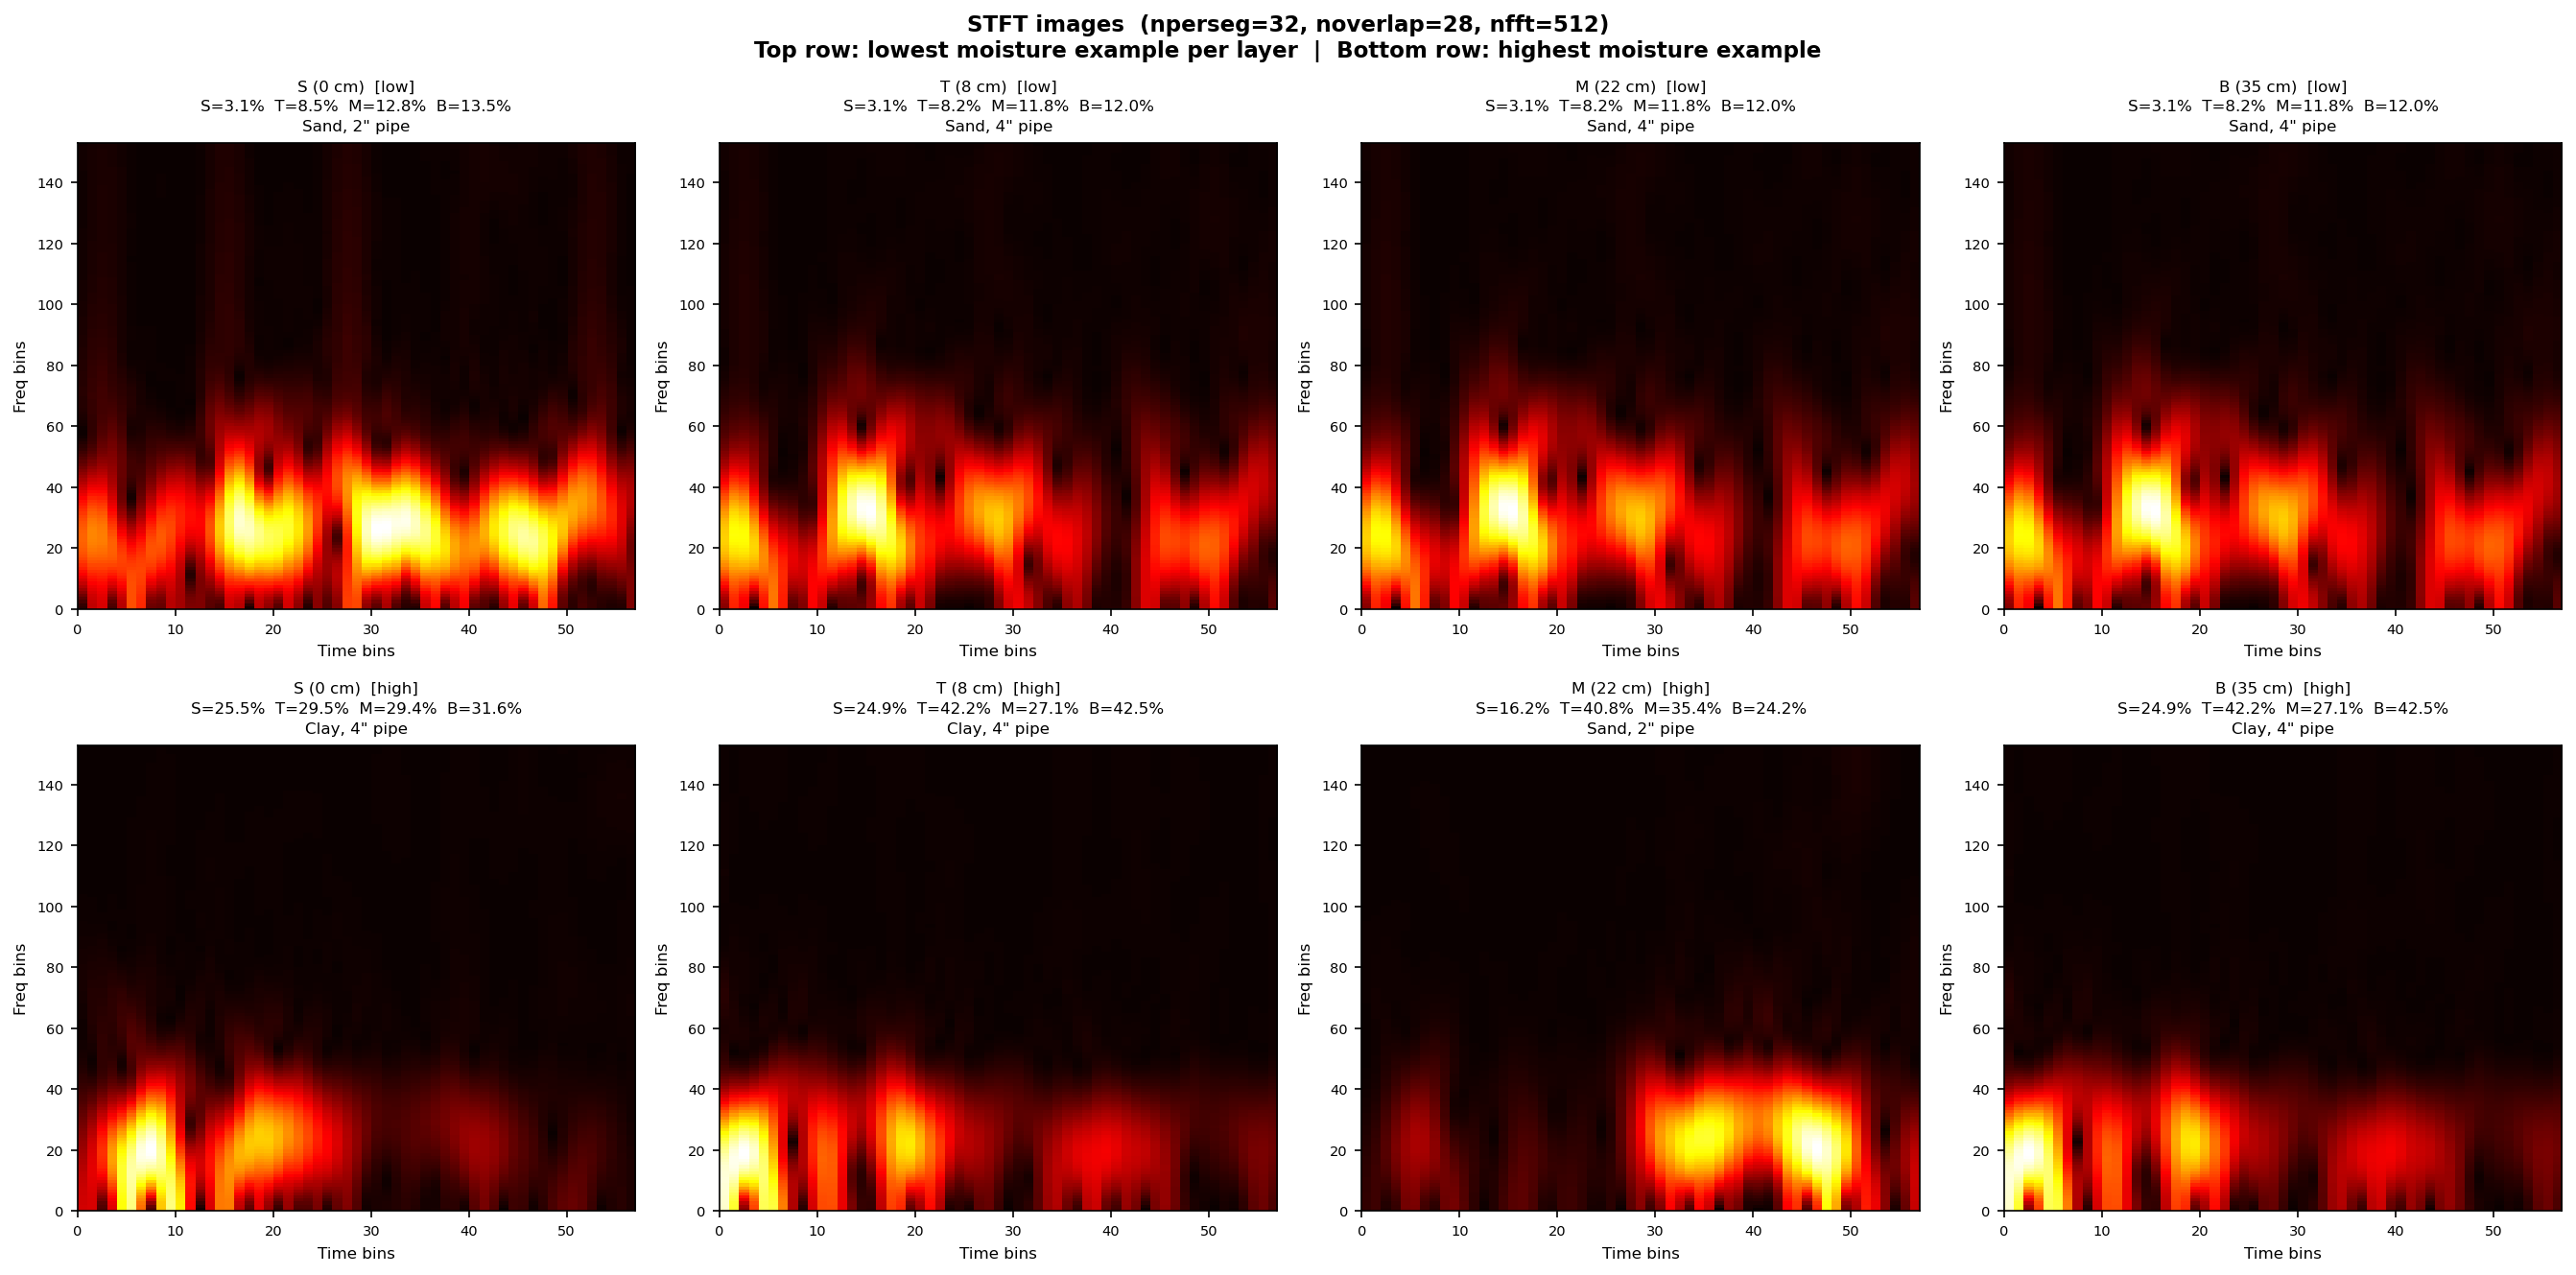
\includegraphics[width=\linewidth]{fig2_stft_samples}
    \caption{STFT spectrograms for two representative samples: low moisture (left) and high moisture (right), for each experimental condition. High moisture delays reflection arrival (time shift) and suppresses high-frequency energy (attenuation), producing distinct spatial patterns.}
    \label{fig:stft_samples}
\end{figure}

A key design choice is the window length $N_w = 32$, which is smaller than the reference value of 56 used in~\cite{Cao2022}. We found that a shorter window provides better time resolution to separate the pipe reflection (occurring around 10--15~ns) from the box-wall echo, at the cost of reduced frequency resolution; this trade-off favors time localization for the present geometry.

\subsection{Condition-aware CNN}
\label{sec:cacnn}

The base 2D CNN processes the STFT spectrogram with three convolutional blocks followed by global average pooling:
\begin{align}
    \mathbf{f} &= \text{AvgPool}\big(\text{Conv}_{64}(\text{Conv}_{32}(\text{Conv}_{16}(\mathbf{X})))\big)
\end{align}
Each convolutional block consists of a $3\times3$ convolution, batch normalization, ReLU activation, and $2\times2$ max-pooling. The global average pooling yields a 512-dimensional feature vector $\mathbf{f} \in \mathbb{R}^{512}$.

For the condition-aware variant, the soil type (2 classes: sand, sandy clay) and pipe diameter (2 classes: 2-in, 4-in) are encoded as one-hot vectors $\mathbf{c}_s \in \{0,1\}^2$ and $\mathbf{c}_p \in \{0,1\}^2$, concatenated to the CNN features:
\begin{equation}
    \hat{\mathbf{y}} = \text{FC}_4\big(\text{ReLU}\big(\text{FC}_{128}([\mathbf{f}; \mathbf{c}_s; \mathbf{c}_p])\big)\big)
\end{equation}
The fully connected regression head maps the concatenated 516-dimensional vector to 4 moisture outputs. Dropout (rate 0.3) is applied before the first FC layer.

The architecture is illustrated in Fig.~\ref{fig:architecture}. The rationale for one-hot condition encoding rather than embedding is that soil type and pipe diameter are mutually exclusive categorical variables with interpretable identities; the one-hot representation makes the network's condition dependence explicit.

\begin{figure}[htbp]
    \centering
    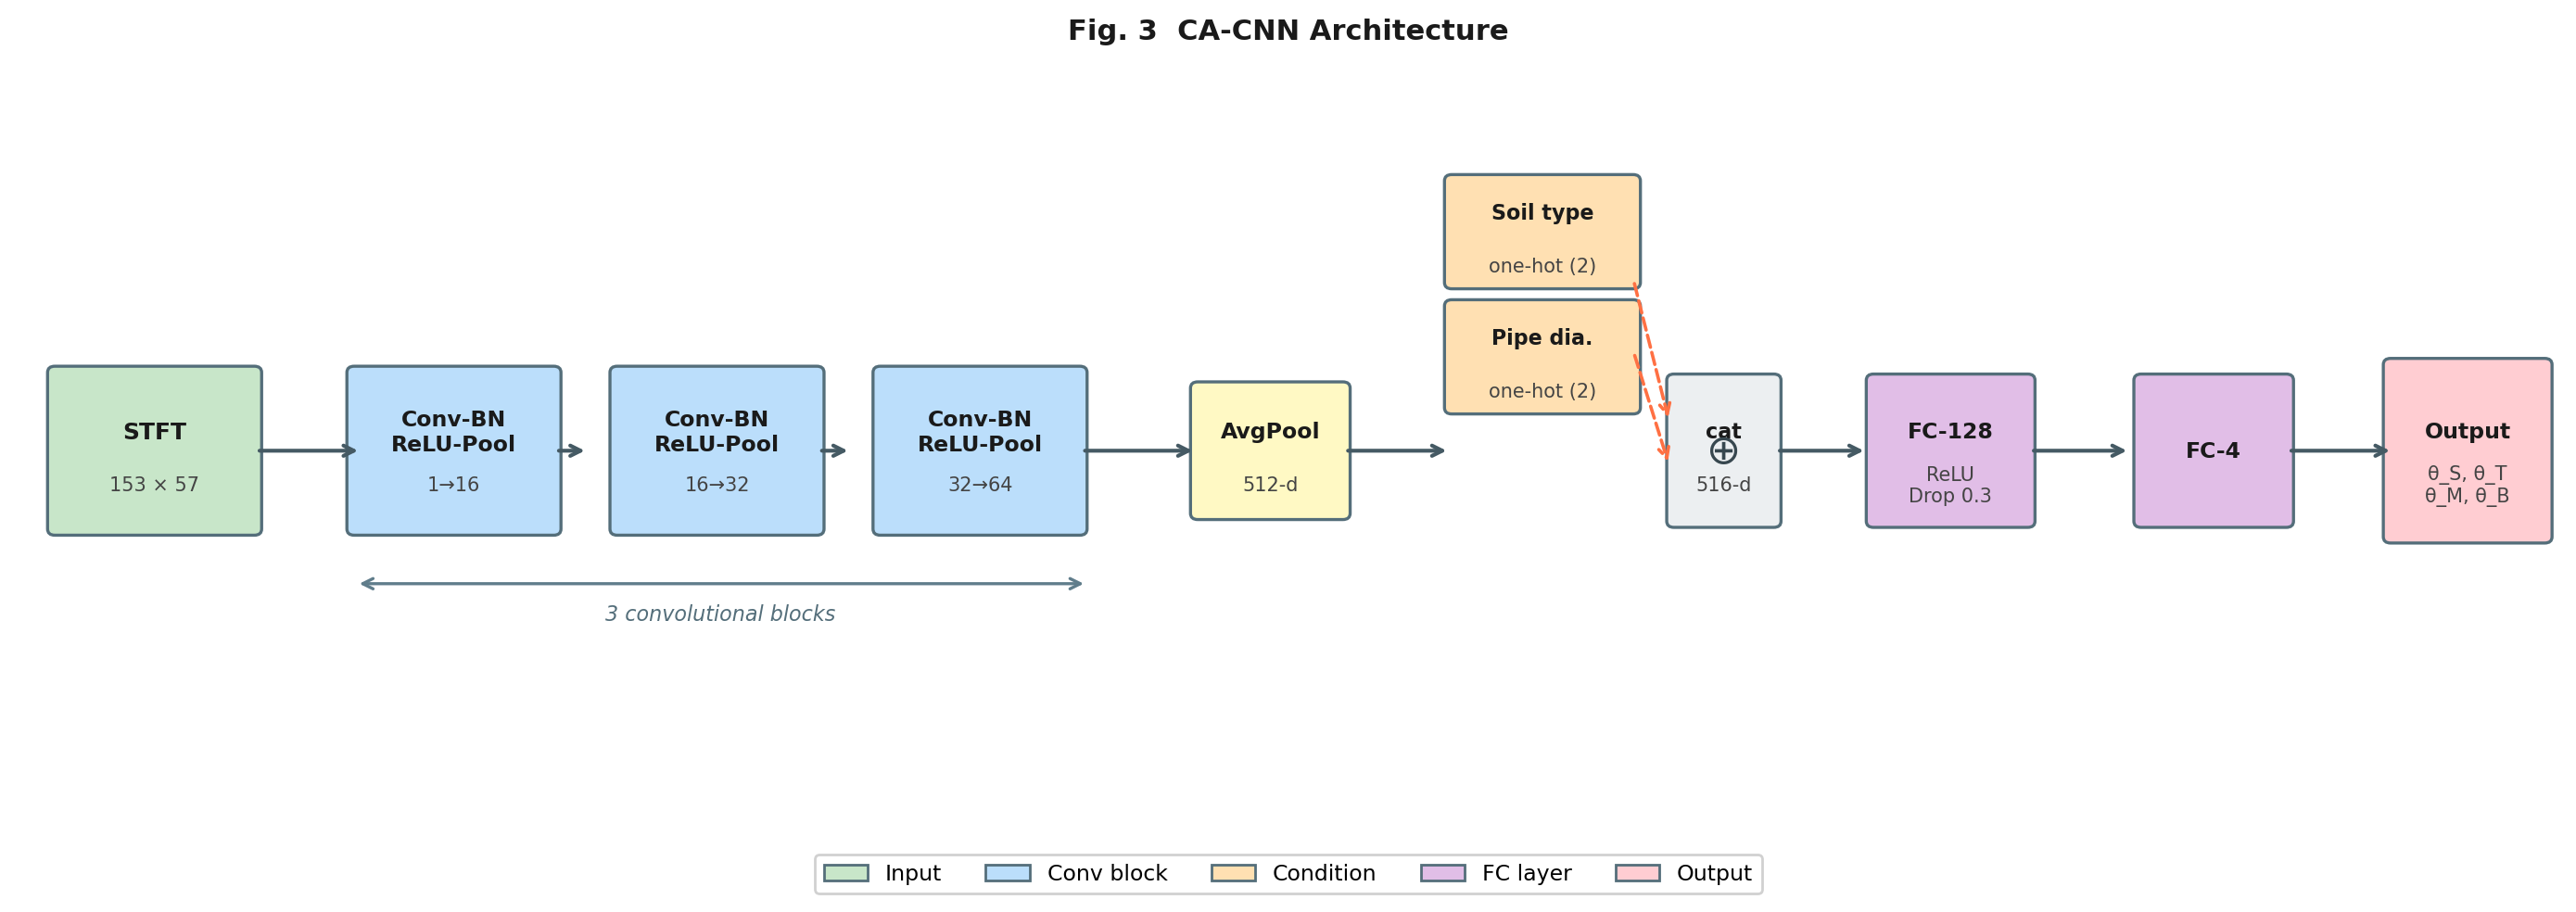
\includegraphics[width=\linewidth]{fig3_architecture}
    \caption{Architecture of the proposed condition-aware CNN. The STFT spectrogram passes through three convolutional blocks (Conv-BN-ReLU-MaxPool) and global average pooling. The resulting feature vector is concatenated with one-hot encodings of soil type and pipe diameter before two fully connected layers that regress 4 moisture outputs simultaneously.}
    \label{fig:architecture}
\end{figure}

Training hyperparameters: Adam optimizer with initial learning rate $10^{-3}$, reduced by factor $0.5$ when validation loss plateaus for 30 epochs (minimum $10^{-5}$), early stopping with patience 80 epochs, batch size 16, maximum 300 epochs. All training is performed on CPU (no GPU required given the dataset size).

\subsection{Conditional WGAN-GP data augmentation}
\label{sec:gan}

A conditional Wasserstein GAN with gradient penalty (cWGAN-GP) is trained to generate synthetic A-scans conditioned on the experimental metadata and moisture label. The generator $G$ maps a noise vector $\mathbf{z} \in \mathbb{R}^{128}$ concatenated with a condition vector $\mathbf{c} \in \mathbb{R}^8$ to a synthetic A-scan of length 256:
\begin{equation}
    \hat{x} = G([\mathbf{z}; \mathbf{c}]), \quad \mathbf{c} = [\mathbf{c}_s; \mathbf{c}_p; \bar{\boldsymbol{\theta}}]
\end{equation}
where $\bar{\boldsymbol{\theta}} \in \mathbb{R}^4$ is the normalized moisture label vector. The critic $D$ distinguishes real from synthetic A-scans conditioned on the same $\mathbf{c}$. The WGAN-GP objective with gradient penalty coefficient $\lambda = 10$ is:
\begin{equation}
    \mathcal{L} = \underbrace{\mathbb{E}[D(\hat{x}, \mathbf{c})] - \mathbb{E}[D(x, \mathbf{c})]}_{\text{Wasserstein distance}} + \lambda \underbrace{\mathbb{E}\left[(\|\nabla_{\tilde{x}} D(\tilde{x}, \mathbf{c})\|_2 - 1)^2\right]}_{\text{gradient penalty}}
\end{equation}
where $\tilde{x}$ is a random interpolation between real and synthetic samples.

Both $G$ and $D$ are fully connected networks with hidden dimensions $[256, 512, 512, 256]$ and $[512, 256, 128]$ respectively, using LeakyReLU activations ($\alpha = 0.2$). The GAN is trained for 500 epochs with Adam ($\text{lr} = 10^{-4}$, $\beta_1 = 0.5$, $\beta_2 = 0.9$) and 5 critic steps per generator step.

To increase label diversity, synthetic samples are generated with interpolated moisture labels: for each synthetic sample, two real training samples are drawn at random, and the target moisture is a convex combination $\lambda \bar{\boldsymbol{\theta}}_i + (1-\lambda)\bar{\boldsymbol{\theta}}_j$ with $\lambda \sim \text{Uniform}(0.3, 0.7)$. Within each fold, the GAN is trained on the training split only, and $2\times$ the training set size of synthetic samples is generated and appended before training the CA-CNN. This prevents any information leakage from the validation fold into the augmented data.

The key motivation for augmenting in the A-scan domain rather than the STFT spectrogram domain is that STFT pixels represent physical observables: the horizontal axis encodes arrival time (causally related to permittivity and depth), and the vertical axis encodes frequency (related to attenuation). Geometric transforms such as horizontal shifts or vertical blurs would alter these physical relationships and potentially associate incorrect moisture labels with the transformed images. We test this hypothesis directly in Section~\ref{sec:ablation_aug}.


%% ============================================================
\section{Results}
\label{sec:results}
%% ============================================================

\subsection{Progressive model comparison}
\label{sec:main_results}

Table~\ref{tab:main_results} presents the cross-validated $R^2$ for each depth layer and the average across all four depths, for all six model variants. The proposed method (Row 6) achieves $R^2 = 0.825$, an improvement of 14.0 pp over the 1D CNN raw A-scan baseline (Row 1).

\begin{table}[htbp]
\centering
\caption{Cross-validated $R^2$ (5-fold) for all model variants. S: surface (0~cm), T: top (8~cm), M: middle (22~cm), B: bottom (35~cm). $\pm$std: standard deviation of fold-averaged $R^2$ across five folds.}
\label{tab:main_results}
\begin{tabular}{lcccccc}
\toprule
Model & S & T & M & B & Avg $R^2$ & $\pm$std \\
\midrule
1D CNN (raw A-scan)              & 0.734 & 0.638 & 0.674 & 0.695 & 0.685 & 0.052 \\
CA-1D CNN (raw A-scan)           & 0.730 & 0.664 & 0.631 & 0.720 & 0.686 & 0.057 \\
STFT + 2D CNN                    & 0.870 & 0.754 & 0.743 & 0.820 & 0.797 & 0.056 \\
STFT + CA-2D CNN                 & 0.853 & 0.800 & 0.781 & 0.828 & 0.816 & 0.056 \\
STFT + CA-2D CNN + noise aug.    & 0.839 & 0.744 & 0.785 & 0.834 & 0.801 & 0.055 \\
STFT + CA-2D CNN + cWGAN-GP\textsuperscript{$\star$} & \textbf{0.884} & \textbf{0.764} & \textbf{0.811} & \textbf{0.843} & \textbf{0.825} & \textbf{0.051} \\
\bottomrule
\end{tabular}
\\ \smallskip
\small\textsuperscript{$\star$}Proposed method.
\end{table}

Several observations follow from Table~\ref{tab:main_results}. First, adding a condition head to the 1D CNN yields no improvement (0.685 $\to$ 0.686), while adding the same head to the STFT CNN yields a consistent improvement (0.797 $\to$ 0.816). This confirms that the benefit of condition encoding is contingent on a rich input representation: the 1D CNN cannot extract features that the condition head can meaningfully complement. Second, simple Gaussian noise augmentation slightly reduces performance (0.816 $\to$ 0.801), while cWGAN-GP augmentation improves it (0.816 $\to$ 0.825). The difference is discussed further in Section~\ref{sec:ablation_aug}.

The T-layer (8~cm) consistently shows the lowest $R^2$ across all models. This layer receives contributions from both the near-surface (S) and the pipe-interaction zone, making its signal more sensitive to measurement noise and geometric variability between experiments.

\begin{figure}[htbp]
    \centering
    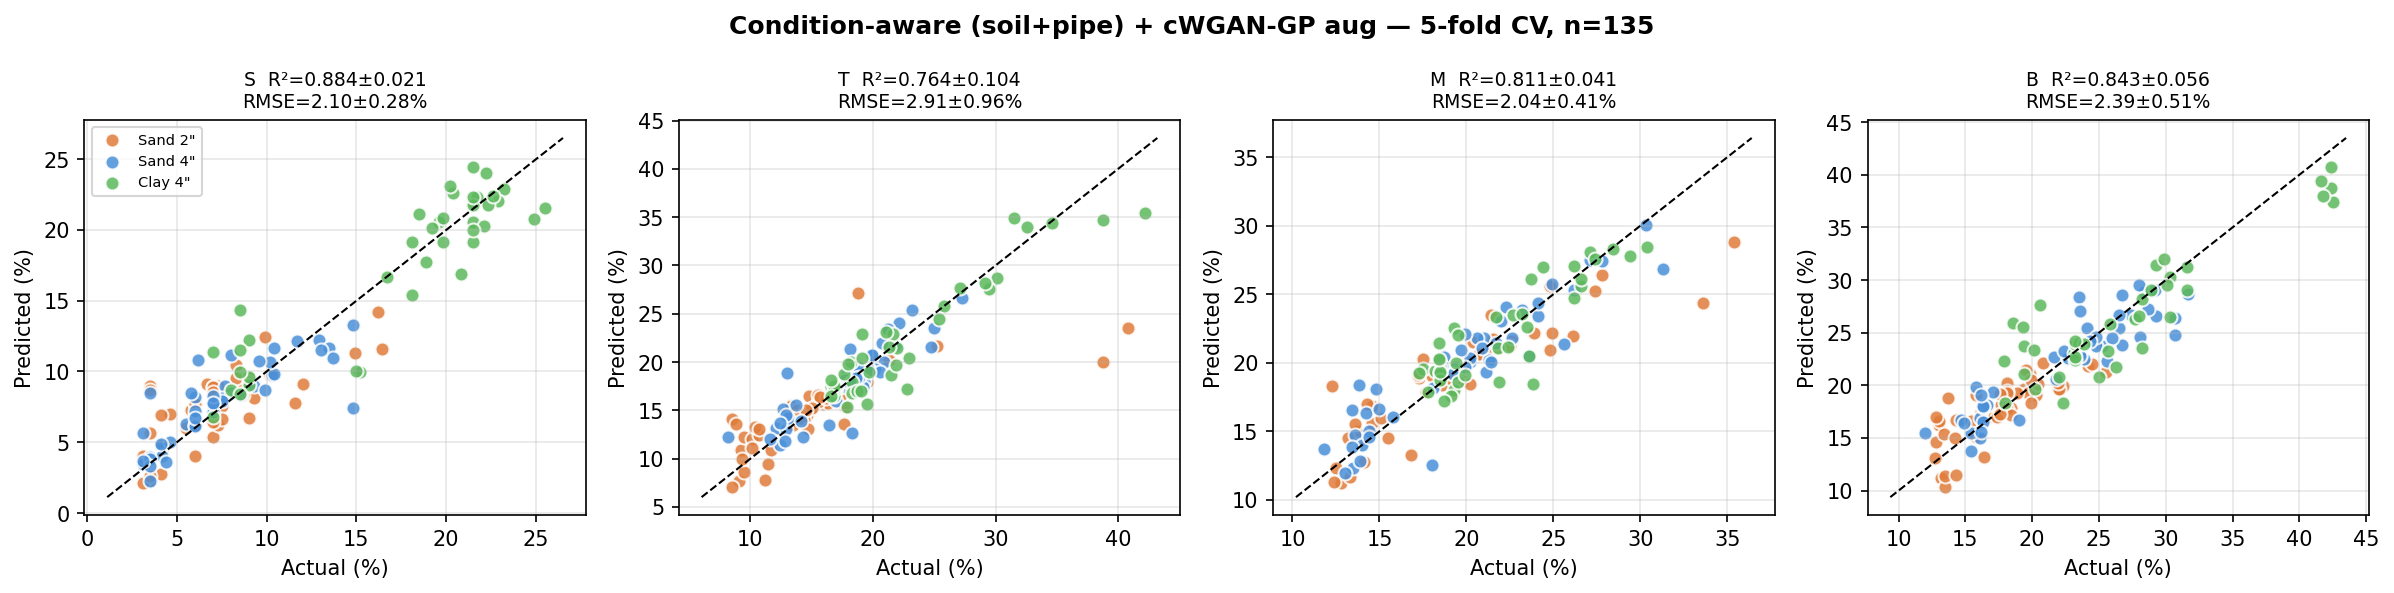
\includegraphics[width=\linewidth]{fig5_scatter}
    \caption{Predicted vs. actual volumetric water content (\%VWC) for the proposed method (STFT + CA-CNN + cWGAN-GP) across all four depths. Each point represents one out-of-fold prediction; color encodes the experimental condition. Dashed line: ideal prediction ($y = x$).}
    \label{fig:scatter}
\end{figure}

\subsection{Ablation study: STFT versus raw A-scan}
\label{sec:ablation_stft}

The 1D CNN and CA-1D CNN results isolate the contribution of the STFT representation. The STFT advantage over the plain CNN baseline is $+0.112$ $R^2$ (0.797 vs. 0.685), and over the CA-CNN baseline with the same condition head is $+0.130$ $R^2$ (0.816 vs. 0.686).

The absence of any benefit from the condition head on the 1D CNN (0.685 $\to$ 0.686) is an informative negative result: it shows that the network cannot leverage known metadata when the signal representation is not rich enough to form features the metadata can interact with. In contrast, the STFT representation encodes moisture effects as 2D spatial patterns, and the condition head allows the network to attribute these patterns to the correct soil type and geometry, explaining why the same head yields $+0.019$ $R^2$ on the STFT baseline.

\subsection{Ablation study: augmentation domain}
\label{sec:ablation_aug}

Table~\ref{tab:aug_ablation} compares five standard image-domain augmentations applied to the STFT spectrogram against the cWGAN-GP augmentation applied in the A-scan domain.

\begin{table}[htbp]
\centering
\caption{Augmentation ablation: average $R^2$ for the CA-2D CNN with different augmentation strategies. All image-domain augmentations are applied to the STFT spectrogram; cWGAN-GP is applied to raw A-scans before STFT conversion.}
\label{tab:aug_ablation}
\begin{tabular}{lcc}
\toprule
Augmentation & Avg $R^2$ & $\Delta$ vs. No aug. \\
\midrule
No augmentation              & 0.816 & --- \\
\midrule
\multicolumn{3}{l}{\textit{Image-domain augmentations (applied to STFT)}} \\
Horizontal shift             & 0.710 & $-0.106$ \\
Brightness / contrast        & 0.698 & $-0.118$ \\
Gaussian blur                & 0.722 & $-0.094$ \\
Gaussian noise               & 0.711 & $-0.105$ \\
CLAHE                        & 0.695 & $-0.121$ \\
\midrule
\multicolumn{3}{l}{\textit{Signal-domain augmentation (applied to raw A-scan)}} \\
cWGAN-GP (proposed)\textsuperscript{$\star$} & \textbf{0.825} & $+0.009$ \\
\bottomrule
\end{tabular}
\end{table}

All five image-domain augmentations degrade performance significantly, with CLAHE producing the largest drop ($-0.121$). This result confirms the central hypothesis of this paper: STFT spectrogram pixels encode physically meaningful quantities (arrival time and frequency-dependent attenuation), and standard image transforms that work well for natural images violate the physical relationships in GPR spectrograms.

Horizontal shift is the most intuitive example: shifting the spectrogram along the time axis would correspond to a change in antenna-to-interface distance, but this change is not accompanied by a corresponding update to the moisture label, creating a label-inconsistent training example. Similarly, brightness and contrast adjustments alter the apparent energy distribution across frequencies without a physical basis, potentially corrupting the frequency-attenuation signature that distinguishes wet from dry soil.

By contrast, cWGAN-GP generates new A-scan signals in the original time domain. The generated signals respect the measurement physics in the sense that they are drawn from the learned distribution of real signals conditioned on the given metadata and moisture level. The STFT conversion is applied afterward, so the resulting spectrogram is physically consistent.

Fig.~\ref{fig:gan_comparison} shows representative real and GAN-generated A-scans and their STFT spectrograms, confirming that the generated signals capture the main spectral features.

\begin{figure}[htbp]
    \centering
    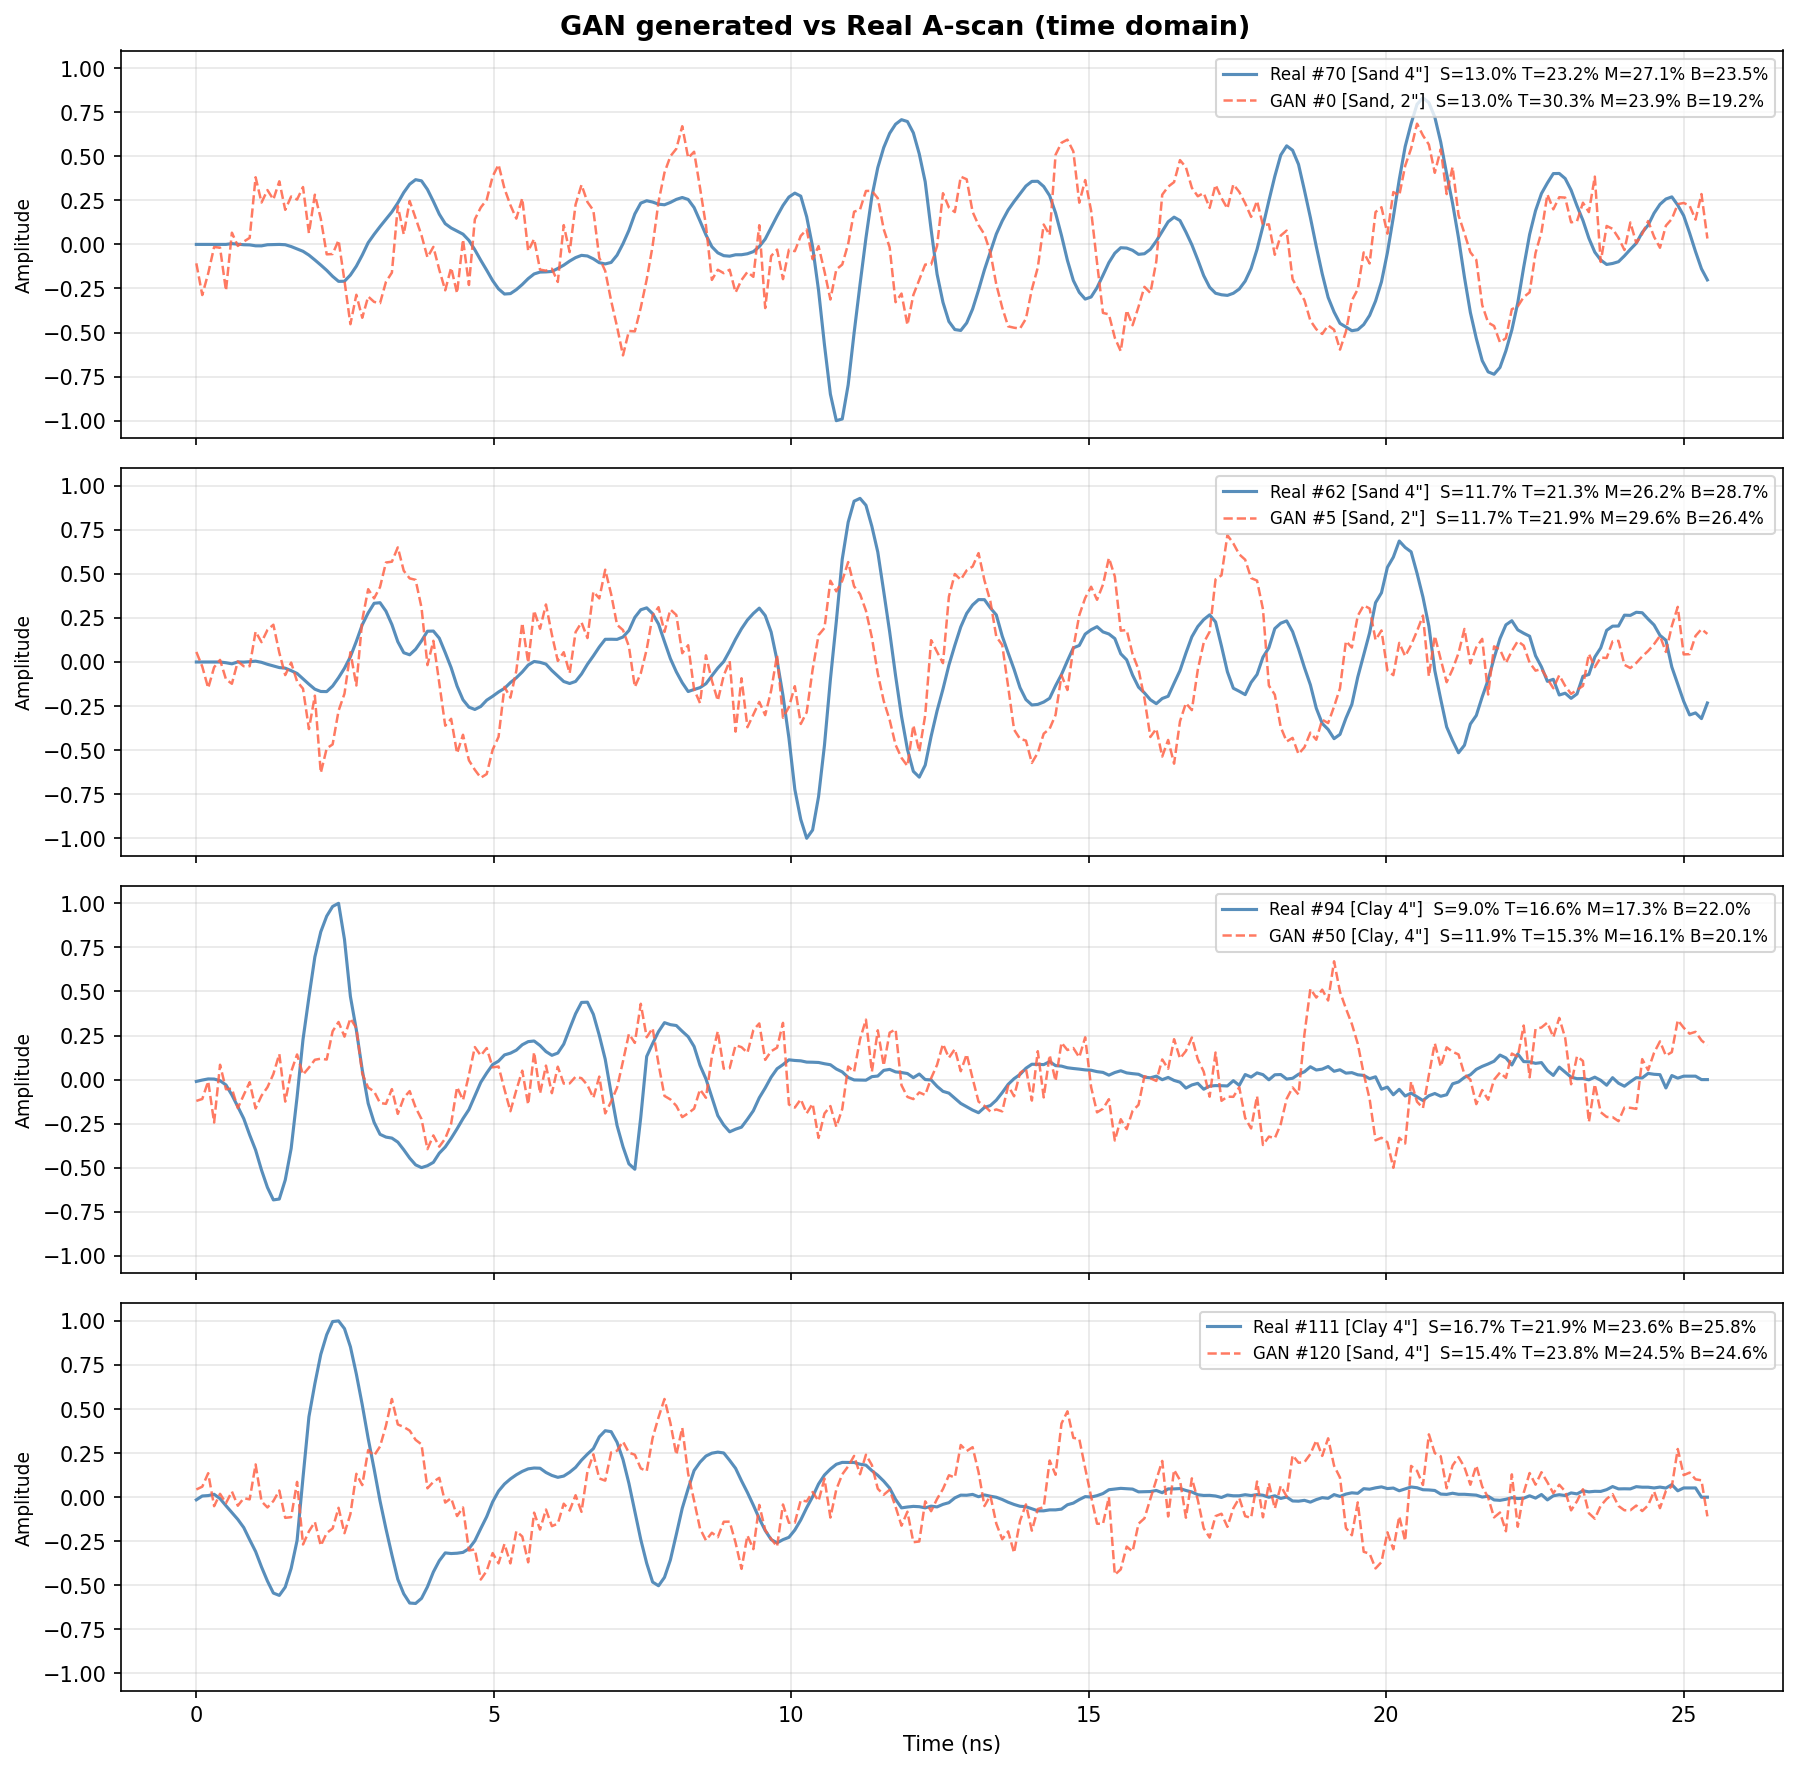
\includegraphics[width=\linewidth]{fig4_gan_comparison}
    \caption{Top: real A-scans (left) vs. GAN-generated A-scans (right) for the same moisture condition. Bottom: corresponding STFT spectrograms. The generated signals reproduce the main reflection event and high-frequency attenuation characteristics of real signals.}
    \label{fig:gan_comparison}
\end{figure}

\subsection{Comparison with physics-based inversion}
\label{sec:physics}

As a non-ML reference, we apply the travel-time inversion described in Section~\ref{sec:related}. The first-break arrival is detected using an envelope-based threshold, and $\varepsilon_r$ is computed assuming the known pipe depth. The Topp equation is then applied to estimate $\theta_v$.

This physics-based method yields $r = 0.545$, $\text{RMSE} = 6.1$\%VWC for the clay condition, where the pipe reflection is relatively prominent. For the sand conditions, the method fails due to interference between the pipe reflection and box-wall echoes, which are not easily separated with a fixed-offset antenna. The proposed ML method does not require knowledge of pipe geometry and achieves $R^2 = 0.825$ across all conditions.


%% ============================================================
\section{Discussion}
\label{sec:discussion}
%% ============================================================

\subsection{Per-layer prediction difficulty}

The consistent ordering $R^2_S > R^2_B > R^2_M > R^2_T$ across all models suggests that the difficulty of moisture prediction is not simply a function of depth. The T-layer (8~cm) is located below the near-surface zone but above the pipe, where the signal is a mixture of contributions from the soil matrix and the top of the pipe's interaction zone. The M-layer (22~cm) is at a comparable depth to the pipe axis and receives contributions from both the soil above and below the pipe. These observations suggest that future work could benefit from architectures that explicitly model the multi-layer nature of the propagation problem.

\subsection{Effect of soil type and pipe diameter on prediction accuracy}

The condition-aware head improves performance over the unconditioned STFT CNN ($+0.019$ $R^2$). However, the absolute improvement is modest, suggesting that the STFT CNN already learns partially separable representations for the three conditions. Future work could explore more expressive condition fusion strategies, such as feature-wise linear modulation (FiLM)~\cite{Perez2018}, which modulates each feature map by condition-dependent scale and shift parameters.

\subsection{Limitations and future directions}

This study has several limitations. The dataset ($n = 135$) is small, and the three experimental conditions represent a limited subset of real-world soil and infrastructure scenarios. The model was trained and tested under the same experimental setup (same tank, same antenna height), which does not evaluate generalization to field conditions. For practical deployment, transfer learning or domain adaptation from simulation-to-real data would be needed. We trained a CycleGAN~\cite{Zhu2017} to translate FDTD-simulated A-scans (gprMax~\cite{Warren2016}, $n_{\text{sim}} = 375$) to the real signal domain; preliminary results show $R^2 = 0.749$ using simulated data with this translation, which remains below the supervised baseline. Closing this simulation-to-real gap is an important future direction.

Additionally, the current experiment uses a single antenna position (fixed-offset, non-displacement). A scanning system would provide a 2D B-scan that encodes additional spatial information and would allow the use of migration processing to improve signal clarity, potentially further improving prediction accuracy.


%% ============================================================
\section{Conclusion}
\label{sec:conclusion}
%% ============================================================

We presented a machine learning pipeline for multi-depth soil moisture prediction from single-pass GPR A-scans. The pipeline consists of STFT-based signal representation, a condition-aware 2D CNN that encodes known deployment metadata, and cWGAN-GP data augmentation in the A-scan domain. On a controlled sandbox dataset with three experimental conditions and 135 samples, the proposed method achieves an average $R^2 = 0.825$ across four depth layers, outperforming a 1D CNN on raw A-scans by 14.0 percentage points.

A key finding of this paper is that the domain of data augmentation matters: five standard image-domain augmentations applied to STFT spectrograms consistently degrade performance, while cWGAN-GP augmentation in the A-scan domain improves it. This result highlights the importance of respecting the physical meaning of signal representations when designing augmentation strategies for GPR and other NDT modalities.

Future work will focus on simulation-to-real transfer to reduce dependence on labeled field data, and extension to scanning acquisitions for 2D moisture mapping.


%% ============================================================
%% References
%% ============================================================

\bibliographystyle{elsarticle-num}
\bibliography{references}

\end{document}
